% !TEX root = flow_head.tex
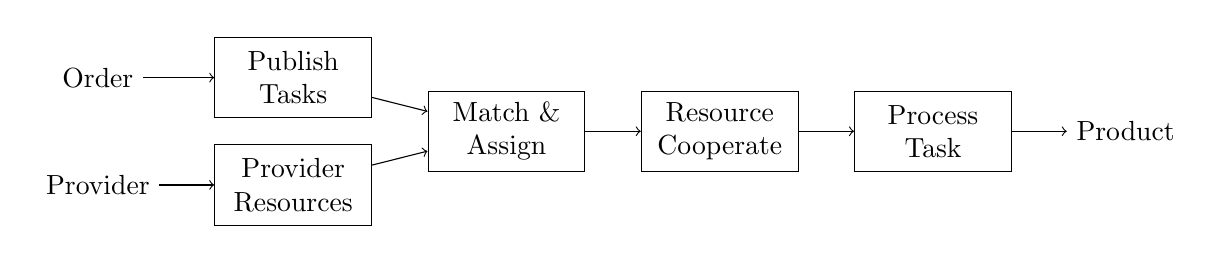
\begin{tikzpicture}[node distance=5mm and 5mm,
square/.style={
% The shape:
rectangle,
draw=black,
minimum size=2.9em,
text width=5em,
text centered
},
circle/.style={
rectangle,minimum size=1em,rounded corners=0.5em,
draw=black
}
]
\matrix[row sep=-1em,column sep=2em] {
% First row:
\node (order) {Order};& \node (task) [square]{Publish Tasks}; & & & & \\
 & &\node (match) [square]{Match \& Assign};&\node (coord) [square] {Resource Cooperate}; & \node (process)[square]{Process Task}; & \node (finish) {Product};\\
\node (provider) {Provider}; & \node (resource) [square]{Provider Resources}; & & & & \\
};
\path (order) edge[->] (task) (task) edge[->] (match) (match) edge[->] (coord) (coord) edge[->] (process) (process) edge[->] (finish) (provider) edge[->] (resource) (resource) edge[->] (match);
% \path (task) edge[->] (job);
% \node (ui1) [nonterminal] {unsigned integer};
% \node (dot) [terminal,right=of ui1] {.};
% \node (digit) [terminal,right=of dot] {digit};
% \node (E) [terminal,right=of digit] {E};
% \node (plus) [terminal,above right=of E] {+};
% \node (minus) [terminal,below right=of E] {-};
% \node (ui2) [nonterminal,below right=of plus] {unsigned integer};
\end{tikzpicture}